\documentclass{bmd2023p}

\begin{document}

%% Titlepage variables

% Title
\title{Instructions for Preparing a Paper for Bicycle and Motorcycle Dynamics
  2023}

% List authors for the title. Call \addauthor{name}{affiliationID} for every
% author. Authors will appear in the order off calls to \addauthor. Please
% manually specify the correct affiliation ID and an asterisk to the
% corresponding author
\addauthor{Firstname1 A. Lastname1}{1}
\addauthor{Firstname2 B. Lastname2}{2}
\addauthor{Firstname3 C. Lastname3}{2,*}

% List authors with only initials for given names, displays only in footer.
\authorfooter{Lastname1, F. A., Lastname2, F. B., \& Lastname3, F. C.}

% List affiliations. Call \addaffiliation{id}{name}{EmailOrcidString} once for
% every distinct institution, where id specifies the affiliation ID (ensure
% that this corresponds to the IDs used with \addauthor), name specifies the
% affiliation name, and EmailOrcidString is a string listing emails and ORCIDs
% (optional) affiliated with this affiliation separating mail and ORCID using a
% comma and different author credentials using a semicolon.

\addaffiliation{1}{Department of Engineering, University of Technology, The Netherlands}{f.a.lastname1@uot.nl, ORCID 1111-1111-1111-1111}
\addaffiliation{2}{Department of Engineering, University of Technology, Germany}{f.b.lastname2@uot.de, ORCID 2222-2222-2222-2222; f.c.lastname3@uot.de, ORCID 3333-3333-3333-3333}

% The following variables will be updated by the publisher, do not edit.
\doi{XX.XXXX/XX.XXXX}
\year{2023}
\editor{Firstname Lastname}
\submitteddate{dd/mm/yyyy}
\accepteddate{dd/mm/yyyy}
\publisheddate{dd/mm/yyyy}
\citation{}
\issn{2667-2812}
% End publisher variables.

%% End titlepage variables

\maketitle

\section*{Abstract:}
The abstract must fit on this title page and should not include figures,
tables, or citations. The abstract has the section heading \textbf{Abstract:},
bold 11~pt Times New Roman, and the abstract text should be written in Times
New Roman, 10~pt. The primary paper contents should start on the second page.

%% Keywords. Call \addKeywords and provide your keywords of joice separated by a semicolon.
\addKeywords{Keyword1; Keyword2; Keyword3; Keyword4; Keyword5; Keyword6}

% New page after the abstract.
\newpage
\pagestyle{headings}

\section*{Introduction}
Authors are requested to upload a paper of 6 to 12 pages (including references
and figures) to the Orvium web site by the stated date in the call for papers.
Please upload your finished manuscript as \verb|.odt|, \verb|.docx|. or zipped
LaTeX project.  PDFs will not be accepted. For LaTeX documents, upload a single
ZIP file that includes the minimum set of source files needed to build a PDF.
The ZIP file should be named using the following pattern
\verb|Surname1Surname2Surname3_paper.zip|. The primary LaTeX file should be
named \verb|paper.tex| and should reside in the root of the ZIP file directory
tree or under the only top level directory, e.g.  \verb|paper/paper.tex|.
Orvium compatible LaTeX packages are listed in the \verb|bmd2023p.cls| file;
use of other packages may not function with Orvium.

The paper must be written in English. It must contain the names, affiliations,
and e-mail addresses of the authors. Do not edit the list of publisher
variables. The paper size is European A4 (21 x 29.7~cm). The left and right
margins are 1.27~cm, the top margin (not including the header) is 2.5~cm, and
the bottom margin is 1.9~cm. The title should be in Times New Roman 18~pt, and
may extend over more than one line. The author's name or authors' names should
be in Times New Roman 10~pt and the affiliation should be in 8~pt. Section
headings are in Times New Roman 11~pt and the primary text is in Times New
Roman 10~pt. All of these fonts are already set and should not be edited. Only
use \verb|\section| and \verb|\subsection| for sectioning the paper's contents.

\section*{Equations, Figures, and Tables}

Equations should be numbered continuously according to the format shown in
Equation~(\ref{eq:equ1}):
\begin{equation} \label{eq:equ1}
  e^{i\pi} + 1 = 0,
\end{equation}
where the unknown symbols are explained after the equation.

Figures, graphs, and tables must be included using the same style as in
Figure~\ref{fig:fig1} and Table~\ref{tab:tab1}. Both figures and tables should
be centered on the page. Use of at least 300~dpi resolution for images and line
art is required, 1~px wide lines in figures should be avoided as they may
become invisible in print.

\begin{figure}[ht]
  \begin{center}
    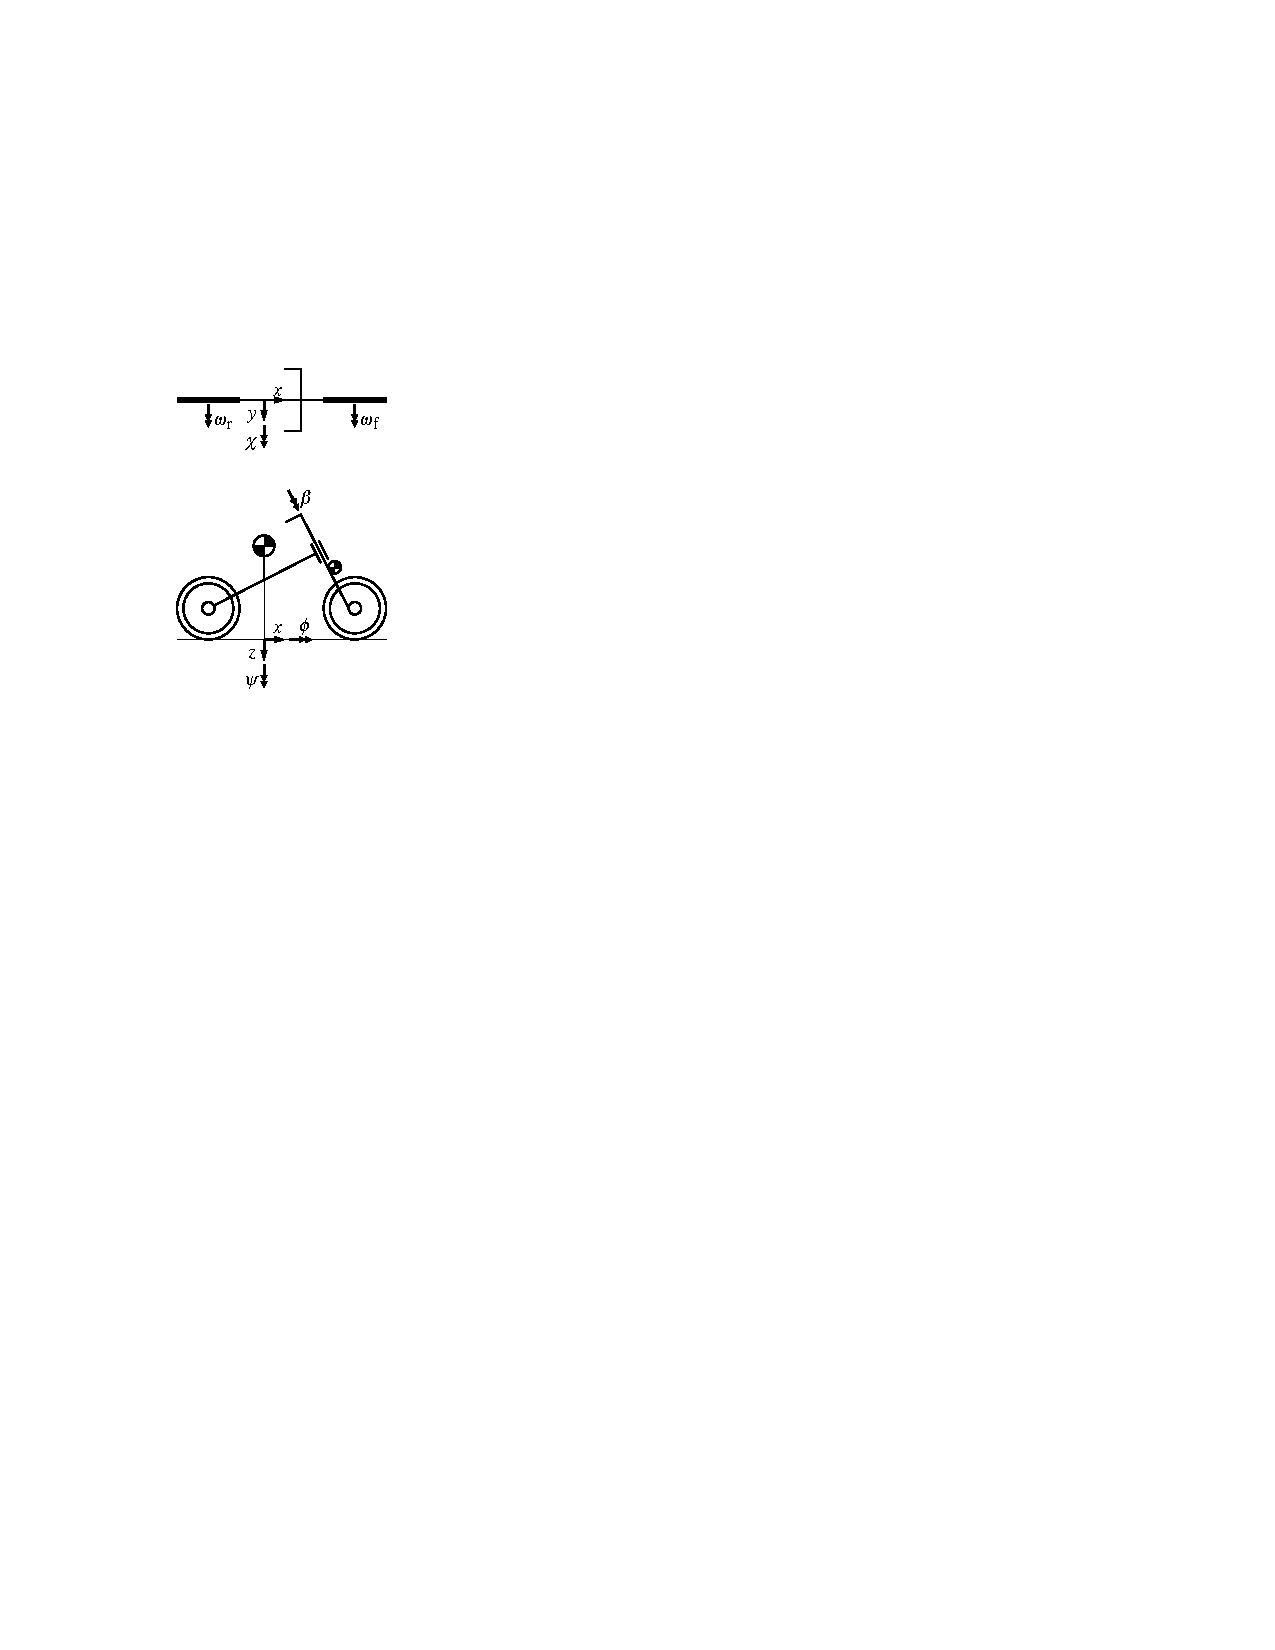
\includegraphics[width=55mm]{figure1}
    \caption{An example of a figure caption. Use 10~pt Times New Roman. Use the
      same style for the tables.}
    \label{fig:fig1}
  \end{center}
\end{figure}

\begin{table}[ht]
  \begin{center}
    \caption{Example of a table with a short caption.} \label{tab:tab1}
    \begin{tabular}{|c|ccc|}
      \hline
      &  $x$  &  $y$  &  $z$ \\
      \hline
      $x'$  &  $\alpha_1$ & $\beta_1$ & $\gamma_1$ \\
      $y'$  &  $\alpha_2$ & $\beta_2$ & $\gamma_2$ \\
      $z'$  &  $\alpha_3$ & $\beta_3$ & $\gamma_3$ \\
      \hline
    \end{tabular}
  \end{center}
\end{table}

\section*{Bibliography}

Bibliographical citations should be written in alphabetical order in the
\textbf{References} section at the end of the document and use the APA citation
system and the APA format. See the \textbf{References} section below, where
\citep{Pac02} exemplifies the case of a textbook, \citep{Ber07} is an article
in a conference proceedings, and \citep{Sha71} is an article in a journal. Make
use of the \verb|natbib| package with \verb|\citep{}| or \verb|\citet{}| for
citations. If using a \verb|.bib| file, use the \verb|apalike| bibliography
style to get APA formatting.

\section*{Conclusion}

We very much look forward to welcoming you in Delft! Best wishes and the
warmest regards from the Organizing Committee of Bicycle and Motorcycle
Dynamics 2023.

% The following manual bibliography declaration is supported:
\begin{thebibliography}{9}
  \bibitem[Bertolazzi et al., 2007]{Ber07} Bertolazzi, E., Biral, F., Da~Lio,
    M., \& Cossalter, V. (2007, June 25--28), The influence of rider's upper
    body motions on motorcycle minimum time maneuvering. In C.~L.~Bottasso,
    P.~Masarati, \& L.~Trainelli (Eds.), \textit{Proceedings, Multibody
    Dynamics 2007, ECCOMAS Thematic Conference}, Politecnico di Milano, Milano,
    Italy, 15.
  \bibitem[Pacejka, 2002]{Pac02} Pacejka, H.~B., (2002). \textit{Tyre and
    Vehicle Dynamics}.  Butterworth and Heinemann, Oxford.
  \bibitem[Sharp, 1971]{Sha71} Sharp, R.~S. (1971). The stability and control
    of motorcycles.
    \textit{Proceedings of the IMechE, Part C, Journal of Mechanical
    Engineering Science}, \textit{13}, 316--329.
\end{thebibliography}

% If you instead use a bib file, remove the
% \begin{thebibliography}...\end{thebibliography} environment above and
% uncomment the following lines to use the apalike style with a bib file, e.g.
% references.bib.
%\bibliographystyle{apalike}
%\bibliography{references.bib}

\end{document}
